\chapter{Introduction and Background}
\label{01intro}

% Some stuff about things.\cite{example-citation} Some more things. 

% Adding in-line citations to my published work using the bibentry package

% CyGNAL:

% - \bibentry{sufi_multiplexed_2021}

% scRNA-seq:

% - \bibentry{cardoso_rodriguez_single-cell_2023}

\section{Significance and Characteristics of Colorectal Cancer}

\acrlong{crc} (\acrshort{crc}) is generally defined as an adenocarcinoma originating from the epithelial lining of the colon or rectum. Despite lowered incidence and mortality rates in recent years \cite{cronin_annual_2022}, \acrshort{crc} is the third most common malignancy worldwide, claiming over 900,000 lives every year \cite{morgan_global_2023}.
% \colorbox{yellow}{EXPAND THIS FURTHER to get rid of bracketed text and add more breathing space. probably no need to expand in terms of info re epidemiology, staging, ....}

The canonical model of \acrshort{crc} pathogenesis is the polyp to adenocarcinoma progression. Originally described at the end of the 20\textsuperscript{th} century by \emph{Fearon and Vogelstein} \cite{fearon_genetic_1990} it is understood to present an initial phase where benign hyperproliferative polyps, often harbouring mutations in the \emph{Wnt} signalling pathway (most commonly in the \emph{APC} gene \cite{aghabozorgi_role_2019}), eventually acquire additional oncogenic mutations that result in malignant \acrshort{crc} (Figure \ref{fig:1crc}). Some of the most common oncogenic mutations target \emph{KRAS}, an oncogene that regulates epithelial proliferation, and \emph{TP53}, a tumour suppressor that normally acts as a gatekeeper of the hyperproliferative polyps \cite{fearon_genetic_1990,armaghany_genetic_2012}. 

Furthermore, the development of \acrshort{crc} also involves the local \acrlong{tme} (\acrshort{tme}), whereby the mutated epithelial cells orchestrate changes in the local inflammatory and stromal niches \cite{peddareddigari_tumor_2010}.

\begin{figure} 
    \centering
    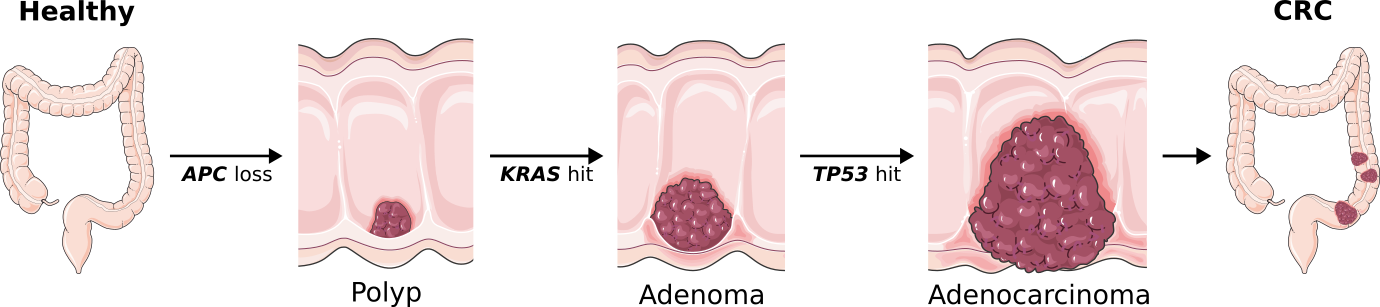
\includegraphics{01intro/figs/1BIO_CRC.png}
    \caption{something something on the canconical model of crc progression. mutations are an introduction into those used in our model. Still missing more muts that should probably be added to the figure.}
    \label{fig:1crc}
\end{figure}
% \addtocounter{figure}{-1}
\cite{van_de_wetering_-catenintcf-4_2002}
% oncogenic mutations targeting \textit{Apc}, \textit{Kras}, \textit{Braf}, \textit{Smad4}, and/or \textit{Trp53} constitute intrinsic cues that induce a crypt-progenitor phenotype in CRC cells \cite{van_de_wetering_-catenintcf-4_2002}

\subsection{The Colonic Epithelium and Colon Stem Cells}

% \colorbox{yellow}{THIS NEEDS SOME KIND OF FORESHADOWING RE LANDSCAPES and CANCER AS PLASTICITY DISEASE}

% \subsubsection{Figure on CRC hallmarks/development}
% \subsubsection{Figure on the colonic epithelia stem niche and its support and changes in CRC}
% something like \colorbox{yellow}{Armaghany et al 2012}
% \emph{This figure will be like that one on the SI vs colon from the Beumer and Clevers 2021 review, but with the right most panel being crc state. Also need to introduce the signalling driving the pro and rev csc (acc to literature) \colorbox{yellow}{Sphyris et al 2021}}

The intestinal epithelium comprises an epithelial mono-layer lining the lower gastrointestinal tract that controls nutrient uptake, coordinates metabolism, and shields against pathogens. In a homeostatic setting, intestinal epithelia has an extremely high turnover rate and is organised as distinct cell populations with absorptive or secretory functions, supported by continuously proliferating crypts \cite{bonis_intestinal_2021}. The colon and rectum form the distal end of the gastrointestinal tract and, unlike the longer small intestinal compartment, they experience a higher microbial load, lack villi, and specialise in liquid uptake \cite{kiela_physiology_2016}.

At the base of the colonic crypts reside LGR5\textsuperscript{+} \acrlong{csc}s (\acrshort{csc}s) that give rise to rapidly proliferating Transit Amplifying (TA) cells (Figure \ref{fig:1epi}A). While the specific differentiation trajectories are not yet fully understood, it seems that an Endoplasmic Reticulum (ER) stress response marks the shift from a basal proliferation state into differentiated epithelial states (Figure \ref{fig:1epi}A) \cite{heijmans_er_2013, coleman_er_2019}. Of those differentiated states the most common ones are the enterocytes with an absorptive (also called colonocytes in the colon), and secretory cells such as; mucus-secreting goblet cells, hormone-producing enteroendocrine cells, and immuno-modulatory tuft cells. 

The delicate balance of spatial and temporal control of cell fate is achieved by two opposing gradients between the basal and apical folds of the epithelium, with WNT and NOTCH signalling higher around the CSC-harbouring crypts, and BMP signalling higher towards the apical areas where absorptive cells are (Figure \ref{fig:1epi}A) \cite{bonis_intestinal_2021, beumer_cell_2021}. Continued epithelial renewal is sustained by the CSC population. Characterised by their expression of the LGR5 R-spondin receptor, CSCs are primed to receive converging signalling cues from stromal and intrinsic signals that delineate areas of cell differentiation and proliferation. 

Although this arrangement is kept relatively consistent throughout the lower gastrointestinal tract, organoid models suggest that the architecture of the homeostatic crypt in the colon appears to be, unlike that of the small intestine, more dependent on exogenous stroma-derived WNT ligands and BMP antagonists \cite{sato_long-term_2011, kondo_emerging_2019}. This difference is thought to be driven by secretory cells known as Paneth cells, which reside at the bottom of the crypts in the small intestine but are absent in the colon. Paneth cells support nearby stem cells through the secretion of antimicrobial peptides, WNT and EGF ligands, and juxtacrine NOTCH signalling. In the colon the presence of secretory cells in deeper areas of the crypts has been described \cite{sasaki_reg4_2016}, but it is believed that the niche supporting the stem compartment is mostly orchestrated by the stroma rather than by these Paneth-like Deep Crypt Secretory cells.

\begin{figure}
    \centering
    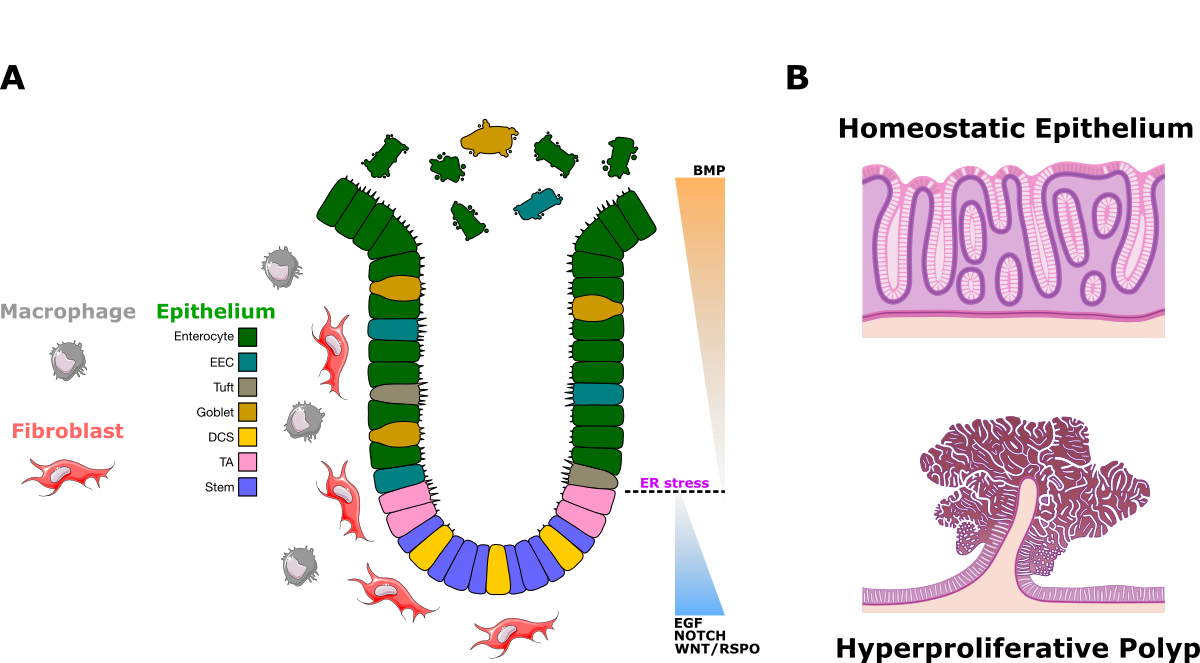
\includegraphics{01intro/figs/1BIO_gutepithelia.png}
    \caption{A) cell types and stem niches and regulation. B) Altered presentation of hyperproliferative polyps when compared to homeostatic colonic epithelium.}
    \label{fig:1epi}
\end{figure}

\subsection{Colorectal Cancer as a Heterocellular Disease}

Genetic alterations in epithelial cells commonly target niche factor signalling hubs that regulate proliferation and differentiation, enabling the CSC compartment to decouple from both pro-survival proliferative signals, and growth-inhibitory cues \cite{sphyris_subversion_2021}. This results in an emancipated and highly proliferative stem-like state (proCSC) that expands beyond the bases of the crypts and dominates the colon epithelium, thus accompanied by a general de-differentiation of the tissue (Figure \ref{fig:1epi}B).

Although it is tempting to think that the expansion of the Colonic Stem Cell (CSC) compartment in CRC is driven by this highly proliferative homogeneous proCSC state, single-cell studies have revealed the presence of additional stem cell states in both homeostatic and CRC epithelium \cite{norkin_single-cell_2020, bankaitis_reserve_2018,barriga_mex3a_2017,bues_deterministic_2022}.
Among them, revival colonic stem cells (revCSC) are emerging as a target of particular interest in cancer research. A rare population in the homeostatic intestine, revCSCs are characterised by \emph{CLU} and \emph{ANXA1} expression and exhibit a less proliferative state that, upon tissue damage, co-opts a phenotype reminiscent of foetal intestinal progenitors to replenish the injured epithelium \cite{ayyaz_single-cell_2019}. 
In the context of CRC, revCSC have been postulated as a putative drug-resistant state that can, after chemotherapy erodes the dominant proCSC state, drive relapse in some CRC patients \cite{rehman_colorectal_2021,alvarez-varela_mex3a_2022}. While the revCSC state has been associated with Hippo and YAP signalling, their exact role in relapse and the mechanisms driving the balance between revival and proliferative CSCs remain unclear.

\emph{A priori} a niche-factor independent compartment, the CRC epithelium comprised mostly of emancipated CSC and proCSC cells is still able to interact and remodel surrounding tissues. This interaction with their environment sustains the view that tumours exist not just as homogeneous clusters of malignant cells, but as a collection of malignant and non-transformed immune and stromal cells \cite{balkwill_tumor_2012}. These untransformed cells constitute the tumour microenvironment (TME), a key factor in most cancers that affect prognosis \cite{calon_stromal_2015} and therefore the subject of intense study in cancer biology and therapy development. 

In their late stage, CRC tumours consist of a complex heterocellular environment in which stromal and immune compartments have been shown to drive cancer cell progression \cite{peddareddigari_tumor_2010,isella_stromal_2015} and response to therapies \cite{tape_heterocellular_2017, toor_immune_2019}.
Cancer associated fibroblasts in particular have been linked with carcinogenesis via secretion of growth factors like EGF, HGF, VEGF and TGF-$\beta$ signalling. In addition, they have also been linked with pro-inflammatory and angiogenic roles, as well as with aiding the CRC tumour in immune evasion and invasion \cite{karagiannis_cancer-associated_2012}.
Within the immune compartment, tumour-associated macrophages are highly abundant, but their functional role within the TME is unclear. There is evidence that they both exhibit pro- and anti-tumour activity, possibly depending on their location within the adenocarcinoma and thei dominance of different macrophage sub-types \cite{martinez_m1_2014}. 
% MArginal periphery apoptosis induction via fas, M1 promoting immune response. OTH, on invasive edge TMAS help tumour, and  M2 downregulate immune response and promote angiogenesis.


\section{Organoids as \textit{in vitro} Models of Colorectal Cancer}

The complexity of CRC can be modelled and studied \emph{in vitro} using organoids, self-organising 3D cellular structures comprising stem and differentiated cells that mimic elements of \emph{in vivo} tissue \cite{huch_modeling_2015,lancaster_disease_2019,almeqdadi_gut_2019}. Mimicking the biology of the \emph{in vivo} setting, gut organoids have a basal stem niche from which differentiated states (with absorptive or secretory functions) derive from; often with an apical lumen within the organoid that accumulates dead cells \cite{sato_single_2009}.

Furthermore, heterotypic settings can be designed wherein colon epithelia organoids are co-cultured with other cell types to model stromal and immune cell-cell interactions \cite{qin_cell-type-specific_2020}. Such settings increase the complexity of organoid systems, allowing for more accurate modelling of \emph{in vivo} tissue architecture and heterotypic interactions \emph{in vitro}. 

In the context of CRC, organoids can be used to characterise both the heterogeneity of the altered colonic epithelium and its interaction with cells of the TME. Furthermore, Patient Derived Organoid (PDO) models are gaining traction as personalised avatars of human tumours \cite{su_efficacy_2023,zapatero_trellis_2023}.

\begin{figure}
    \centering
    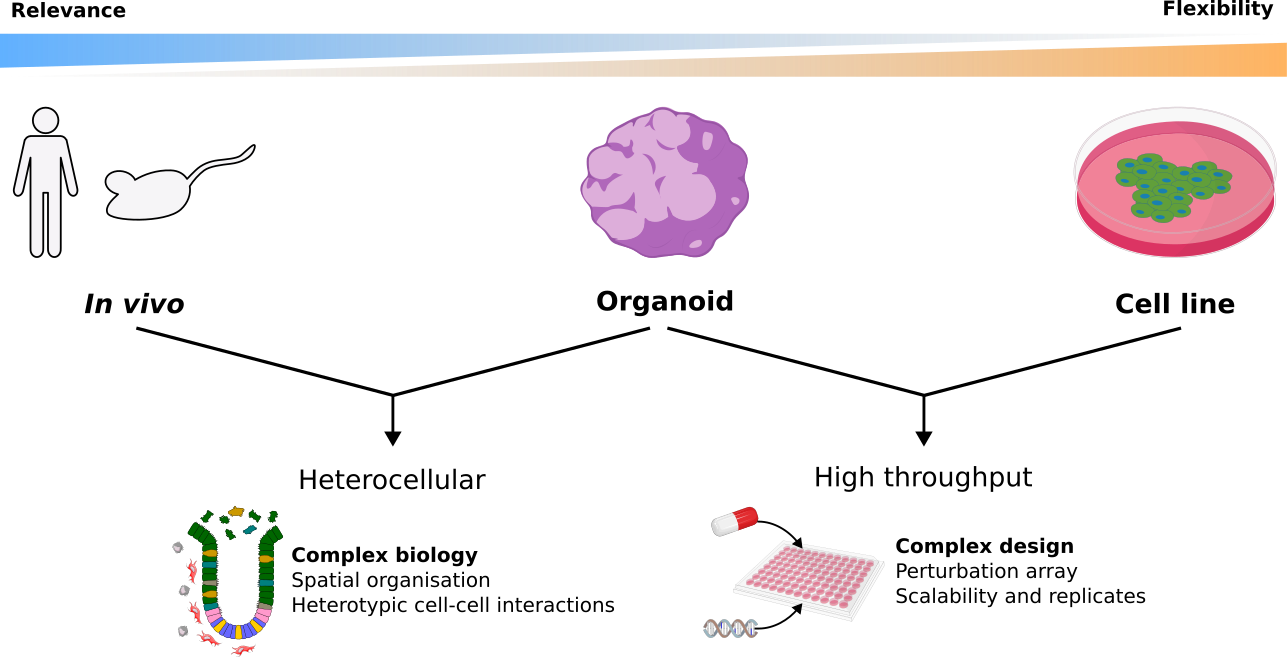
\includegraphics{01intro/figs/1BIO_organoids.png}
    \caption{organoids}
    \label{fig:1org}
\end{figure}

% \subsection{Platforms for High Throughput and Dimensional Models}

Organoids provide a balance between experimental flexibility and physiological relevance. They are complex enough to mimic the heterogeneity of \emph{in vivo} tissue while still being amenable to high-throughput applications \cite{qin_deciphering_2020}. This facilitates high throughput experimentation by allowing for the multiplexing of high numbers of experimental conditions, with for example our custom mass cytometry platform in Sufi \& Qin \textit{et al}. reaching up to 126 plex per run \cite{sufi_multiplexed_2021}.

Recent work by our lab \cite{qin_cell-type-specific_2020} has shown how both CRC genetic perturbations (\textit{shApc}, \textit{Kras\textsuperscript{G12D/+}} and \textit{Trp53\textsuperscript{R172H/–}}) and TME complexity (heterotypic epithelial organoid cultures with fibroblasts and/or macrophages) effect the biology of colonic organoids. Using a custom multivariate mass cytometry platform to analyse post-translational modification (PTM) signalling networks, Qin \textit{et al} \cite{qin_cell-type-specific_2020} found that the distribution of both cellular sub-types and states within the epithelial population changed in a similar and synergic way. They found that both oncogenic and stromal cues resulted in an enrichment of the crypt and stem niches and a reduction of cells in G0 and apoptotic states. Furthermore, their results suggest that the effects of the TME on intracellular epithelial signalling pathways might mechanistically differ from those driven by CRC mutations in the epithelial cells, even if they both share downstream signalling profiles.

This work, featuring multiple axes of variation and replicates within a single experiment, highlights the systematic scalability of organoid models. Moreover, the organoid-inherent heterogeneity coupled with heterotypic cultures justifies comprehensive single-cell analysis to be deconvoluted.
Mature bulk technologies are not poised to leverage heterogeneous 3D organoids; hence, the rapid emergence of single-cell resolution studies in recent years. Single-cell \emph{omic} approaches can deconvolute the different cell types within a heterotypic organoid system as well as resolve particular cell states within each type and even capture cellular interactions within the different compartments \cite{tape_heterocellular_2017}.


\section{Single-Cell \emph{Omic} Technologies}

During this work I leveraged two distinct single-cell technologies to characterise heterocellular organoid models of CRC; mass cytometry (MC) and single-cell RNA sequencing (scRNA-seq). They are both part of the broader family of single-cell \emph{omics} analyses, which have gained traction in characterising cellular heterogeneity at both genotypic and phenotypic levels. 

The concept of \emph{"omics"} is not well defined, but it is commonly understood to describe analyses pertaining to the study of large-scale biological datasets characterising sets of biological molecules from living entities. Some of the most common \emph{omic} studies are the fields of genomics, epigenomics, transcriptomics, and proteomics.
\emph{Omic} information can thus be used to infer cross-\emph{omic} regulatory relationships and decipher causal relations between genotype and phenotype with the right experimental settings.


\subsection{Mass Cytometry (MC)}

MC, also known as Cytometry by Time-Of-Flight (CyTOF), is a technology that merges principles of mass spectometry and flow cytometry to enable single-cell analysis of protein expression. Like flow cytometry, MC is based on tagged antibodies that bind to specific epitopes in cells, but it is able to overcome the issue of florescent spectral overlap by using monoisotopic rare-earth metals instead of fluorophores. The discrete nature of the monoisotopes compared to the broad emission spectra of fluorophores allows for the design of antibody panels that can capture up to \(1\cdot10^2\) features per cell \cite{tracey_cytof_2021}. 

Resolving total protein level information in single-cells is itself incredibly useful, but mass cytometry also excels at resolving post-translational modifications (PTMs) \cite{ochoa_functional_2019}. PTM information often determines a cell's state in relation to the cell cycle, as this process is not really regulated at the gene level but rather by a tight control of different PTM-driven checkpoints \cite{cuijpers_guiding_2018}. This capability also allows for in-depth study of intracellular signalling networks, DNA-damage responses, and apoptosis, and has already been used to characterise both cell-state and oncogene- and stroma-driven signalling changes in murine CRC organoid models \cite{qin_cell-type-specific_2020}.

Coupled with a custom multiplexing platform \cite{sufi_multiplexed_2021} \acrshort{mc} technology can analyse extremely wide experimental systems covering a large number of conditions and replicates, which proves especially useful for drug screening applications \cite{zapatero_trellis_2023}.

However, while powerful in the study of intracellular signalling, \acrlong{mc} struggles to resolve intercellular communication through the complex extracellular interactome of ligands and receptors. In contrast, \acrfull{scrnaseq} technologies can prove extremely useful for this purpose, especially when combined with intercellular cell communication databases such as CellChat \cite{jin_inference_2021} and CellPhoneDB \cite{efremova_cellphonedb_2020}.


\subsection{Single-Cell RNA Sequencing (scRNA-seq)}

With the advent of next generation sequencing (NGS) technologies, bulk-based RNA sequencing approaches were devised that could capture genome-wide transcriptomic information from a whole sample. This mature technology enabled key discoveries across a variety of fields, including tissue development and cancer biology, but its inability to resolve individual cells and their states is a key limitation in systems with complex transcriptional dynamics and multiple cell types \cite{li_bulk_2021}.
scRNA-seq overcame this issue by capturing transcriptomic information at the level of individual cells. Now, a collection of discrete transcriptomic profiles can be pieced together to recapitulate continuous differentiation trajectories, or complex heterocellular systems could now be resolved into their individual cell types \cite{haber_single-cell_2017}. However, while powerful, scRNA-seq comes with significant technical challenges and costs. 

Mature and highly optimised microfluidic droplet-based approaches tend dominate the commercial market, with 10X Genomics offering commercial products \cite{kitzman_haplotypes_2016} that perform the best in terms of UMI and gene / cell detection whilst being a high-throughput application \cite{ding_systematic_2020}.

\begin{figure}
    \centering
    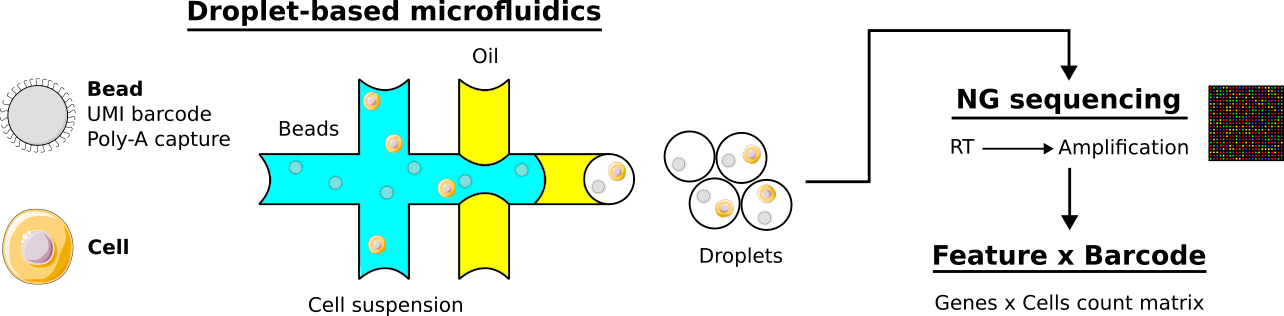
\includegraphics{01intro/figs/1TECH_scRNAseq.png}
    \caption{cell types and stem niches and regulation. NG, next generation (sequencing).RT, reverse transcription. UMI, unique molecular identifier.}
    \label{fig:1tech}
\end{figure}

Droplet-based scRNA-seq methods work by encapsulating individual cells and uniquely tagged beads into water-in-oil droplets, where the cells and beads constitute the dispersed phase and the oil forms the continuous phase encapsulating the droplets \cite{macosko_highly_2015} (Figure \ref{fig:1tech}). During amplification using the poly-A tail capture primers (Figure \ref{fig:1tech}), a unique cellular barcode is added and shared across all products from a single droplet, and a unique molecular identifier (UMI) is also added as a transcript-specific tag before amplification.
Resolving the single-cell level data then relies on only one cell being present in each droplet, so to avoid duplicates a significant percentage of droplets are left empty \cite{abate_beating_2009}. scRNA-seq methods are also characterised by dropout effects, as they capture genes with relatively low yields, resulting in sparse and noisy datasets \cite{qiu_embracing_2020}. 

Despite their good performance and field dominance, high throughput droplet-based microfluidic scRNA-seq approaches still represent a significant monetary burden due to library preparation, which negatively affects scalability and might even, in extreme cases, jeopardise scientific validity by potentially constraining the presence or number of replicates \cite{zimmerman_practical_2021}.
    % \colorbox{yellow}{A practical solution to pseudoreplication bias in single-cell studies} (https://www.nature.com/articles/s41467-021-21038-1) talks about issues derived from the fact that often times not replicates available and that individual cells from the same sample ARE NOT replciates, whereas in DE they are common treated as completely distinct obeservations when comparing clusters.

To overcome this burden, there has been an emergence of microfluidic-free approaches in recent times. Clark \textit{et al.} recently developed PIP-seq \cite{clark_microfluidics-free_2023}, a droplet-based approach based on vortexer emulsification that aims to reduce costs and protocol complexity. By contrast, split-pool barcoding approaches do require a considerable amount of liquid handling steps but promise incredible scalability by using combinatorial split and pooling steps to uniquely barcode at once all cells within a sample \cite{rosenberg_single-cell_2018}.

In the context of CRC, scRNA-seq has been widely used to describe intestinal epithelia \emph{in situ} \cite{haber_single-cell_2017} and even in organoid models, but to date no systematic analysis of colon epithelia across multiple perturbation axes capturing both CRC oncogenic status and changes in the TME has been performed. 

Also known as massively parallel methods, NGS transcriptomics requires the isolation and lysis of cells, reverse transcription of their RNA into cDNA, and then amplification to generate sequencing libraries (Figure \ref{fig:1tech}). Despite being relatively mature technologies, it is still an advancing field, with costs reduction following Moore's Law during the last decade \cite{wetterstrand_dna_2022}.
Emerging third-generation sequencing technologies \cite{check_hayden_genome_2009} are capable of sequencing at the single-molecule level and generally produce reads that are longer than those of NGS approaches \cite{eid_real-time_2009,deamer_three_2016}. Able to also measure multiple \emph{omic} layers \cite{ni_deepsignal_2019}, they are poised to challenge the more common NGS technologies in the future.


\section{Single-Cell \emph{Omic} Data Analysis}

Single-cell technologies generate \emph{omic} scale profiles at the resolution of individual cells, so that complex heterocellular systems like organoids or \textit{in vivo} tissues can be profiled.
However, these approaches produce extremely high dimensional datasets due to the large-scale nature of \emph{omic} data and the single-cell resolution of the technology. Although the large amount of data generated certainly does present a technical challenge, it also allows for a myriad of complex analytical approaches that leverage its complexity and depth to the fullest extent \cite{mincarelli_defining_2018,qin_deciphering_2020}. 

\subsection{The Three Axes of Dimensionality}

% \subsubsection{FIG on data characteristics and general workflow. Also types of analyses for scRNA-seq in specific}
% Big one, review style.
% Convey the info presented in both FIgures 2 and 5 of Xiao's review. Most important from here is the broad pipeline of analysis.
\begin{figure}
    \centering
    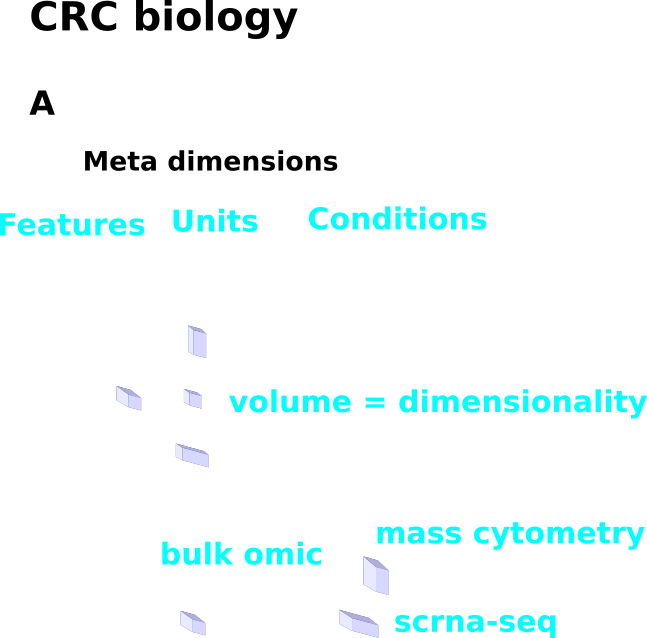
\includegraphics{01intro/figs/1COMP_dims.png}
    \caption{}
    \label{fig:1dims}
\end{figure}


Within the context of \emph{omic} approaches, data dimensionality can be thought of three distinct axes; 1) the number of features to be measured, such as genes or proteins, 2) the number of units whose features are measured, and 3) the number of conditions, groups of units representing a particular biological setting \cite{qin_deciphering_2020}. Thus, a concept of meta-dimensionality is useful to refer to all axes at once.
The unit of measurement is dependent on the methodology used, with bulk methods measuring at the level of whole samples whereas single-cell approaches resolve individual cells. Some spatial \emph{omic} methods fall somewhere in between bulk and single-cell approaches, examining specific regions of a sample containing a small number of cells \cite{vickovic_high-definition_2019,marx_method_2021, williams_introduction_2022}.

Thus, single-cell approaches can generate extremely high-dimensional datasets due to the large-scale nature of \emph{omic} data and the single-cell resolution of the technology. This presents new data analysis challenges that are further compounded when applied to highly scalable models such as organoids that allow for high numbers of conditions to be measured. Machine learning approaches and dimensionality reduction techniques are thus commonly applied to extract meaningful information from high dimensional single-cell data, and, while there is still no uncontested consensus, the more common approaches will be discussed below.
% This has come with added difficulties such as resolving individual cells from complex 3D organoid structures and dealing with the high dimensionality of the resulting data14. 


\subsection{Data Integration}

The essence of data integration is the merging of multiple discrete datasets, and their applications range from batch correction to disjoint cross-modality integration, where modality refers to different sets of measures generally across different \emph{omic} fields.

Of the different types of integration tasks, the most common is between datasets with feature overlap but different units (cells) being measured. This type of integration is needed when datasets are acquired as different events, where generating a combined feature space onto which the cells are projected is relatively straightforward (if indeed necessary at all) and the goal is to remove any technical noise while conserving the biological signal. Data integration approaches range from simple linear methods like mean-centring adjustment commonly used for batch effect correction \cite{hornung_combining_2016}, to more complex approaches such as canonical correlation analysis \cite{butler_integrating_2018} which uses shared anchors to integrate datasets with partially overlapping features. With the later having a tendency towards over-smoothing biological signals, recent methods like STACAS \cite{andreatta_stacas_2021} have been proposed to integrate samples with heterogeneous cell states that might only partially overlap.

Alternatively, sometimes it is necessary to integrate across datasets joint along the cell axis but with different feature sets. A quite common occurrence when dealing with multi-modal techniques, this task can be approached in several ways. The oldest approaches attempted to map the modalities into a shared feature space using cross-omic prior knowledge \cite{chen_assessment_2019}, but these have mostly been replaced by techniques that consider the different modalities to be representations of the same underlying manifold, thus attempting to align the two spaces with techniques such as optimal transport while also optionally incorporating prior knowledge \cite{cao_unsupervised_2020, cao_multi-omics_2022}.

Finally, the most challenging integration tasks are those where there is no overlap between feature or unit spaces. In these cases, integration relies on the assumption that the cells analysed belong to the same underlying manifold of cell states (i.e. they are different snapshots of the same biological process being sampled), and allows for \emph{in silico} generation of cross-omic integrated space from multiple disjoint unimodal datasets and atlases \cite{amodio_magan:_2018,lotfollahi_mapping_2022,cao_multi-omics_2022}.


\subsection{Common Practices for Data Analysis}

% \subsubsection{FIG on data characteristics and general workflow. Also types of analyses for scrnaseq in specific}
% Big one, review style.
% Convey the info presented in both FIgures 2 and 5 of Xiao's review. Most important from here is the broad pipeline of analysis.

% \cite{luecken_current_2019} Classical scrnaseq

% \cite{slovin_single-cell_2021}(https://link.springer.com/protocol/10.1007/978-1-0716-1307-8_19) Review/protocol on the different comp steps of analysis. Idea of nothing being standard

% \cite{heumos_best_2023} Heumos et al 2023: Best practices for single-cell analysis across modalities. MOst recent, from the multiomics angle

\begin{figure}
    \centering
    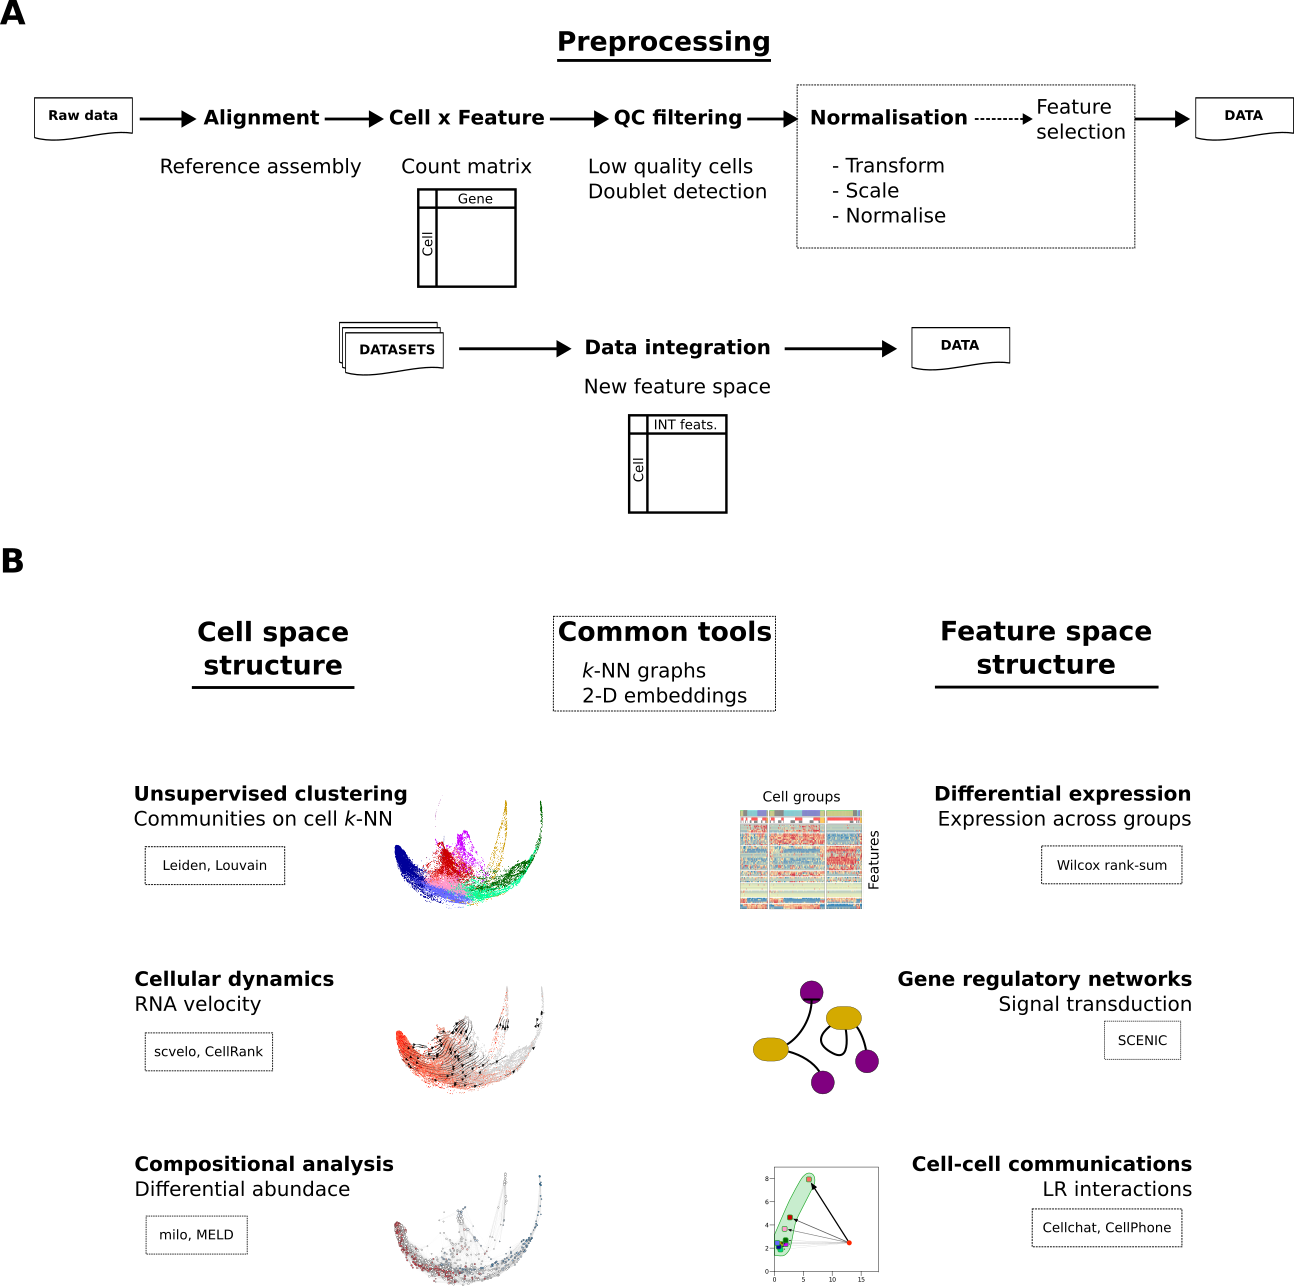
\includegraphics{01intro/figs/1COMP_analysis.png}
    \caption{}
    \label{fig:1pipe}
\end{figure}

Analysis of single-cell omic data is a growing and mostly non-standardised field where a myriad of tools and approaches have been proposed to leverage rich and high-dimensional single-cell omic datasets. Structurally, it is commonly divided between pre-processing and downstream analyses, and while there are some general guidelines and approaches pervasive to the field \cite{luecken_current_2019, heumos_best_2023}, even very established tenets like the unsupervised clustering of cells continue to be debated.

\textbf{Pre-processing} of the data encompasses from more upstream tasks such as sequence alignment and feature normalisation, to further downstream steps like data integration (Figure \ref{fig:1pipe}A), commonly done after a certain degree of exploration of the feature and unit spaces. In the case of scRNA-seq, the first step is to align the sequenced reads against a transcriptome of reference \cite{dobin_star_2013,bray_near-optimal_2016}. This process enables the generation of a count matrix that represents the unit X feature space, i.e. the gene expression detected for each gene (feature) on each cell (unit).

Once the cell X feature matrix has been generated, filtering-based quality control (QC) is performed, whereby cells that do not meet thresholds set on the feature space are removed. Commonly, as part of QC protocols doublet and apoptotic or otherwise compromised cells also get removed.
The filtered data is then transformed and scaled to account for factors that might obscure biological signals, such as differences in cell metrics or feature detection capabilities and sequencing depth. These normalisation steps vary according to the data being analysed, so that for mass cytometry datasets intensities are usually normalised used an inverse hyperbolic sine transform (\(asinh x\)) with a co-factor of \(5\) \cite{bendall_single-cell_2011,guldberg_computational_2023}. For scRNA-seq the approaches range from simpler (and seemingly more robust) log-based transformation \cite{ahlmann-eltze_comparison_2023} and depth-based normalisation \cite{booeshaghi_depth_2022}, to more complex methods like SCTransform \cite{hafemeister_normalization_2019} that use Generalised Linear Methods with Pearson residuals and are able to regress out unwanted sources of variation.

Feature selection is a common pre-processing step that precedes downstream analysis. In the sequencing field, feature selection is commonly limited to selecting highly variable genes, as it is assumed that those will carry relevant biological information and will also speed up compute time by limiting the large feature space. In less feature-rich \emph{omic} technologies, such as mass cytometry, the aim of feature selection is rather a temporary process wherein certain features are used to determine a specific metric (such as nested Boolean gating of cell-cycle associated PTMs to determine cell state \cite{behbehani_single-cell_2012,qin_cell-type-specific_2020}). Often times it is done in conjunction with the normalisation steps commonly performed upstream (Figure \ref{fig:1pipe}A).

If relevant, data integration is commonly performed after the QC and normalisation steps, most commonly with the aim of either removing batch effects between samples or to generate a shared feature space across modalities \cite{cao_multi-omics_2022}. 

Dimensionality reduction (DR) techniques aim to reduce the complexity of the the data while still preserving as much information as possible. If we consider that individual cells belong to a manifold where local structure can be mapped to an Euclidean space our aim would be to preserve distances between cells both in this local space but also at the global level across distant points in the manifold. Principal Component Analysis (PCA) \cite{pearson_liii_1901,jolliffe_principal_2016} was defined in the pre-computational era of the early 20\textsuperscript{th} century and is still commonly used due to it's simplicity and speed. However, PCA is only capable of capturing linear relationships, and thus is generally used as an intermediate DR approach where high dimensional data is compressed to a feature space of \(1\cdot10^1\) to \(1\cdot10^2\). Later DR approaches aim to capture non-linear relationships and to better reflect the underlying manifold, and include methods like Diffusion Maps \cite{coifman_diffusion_2006}, t-SNE \cite{van_der_maaten_visualizing_2008} and UMAP \cite{mcinnes_umap_2020}. While these methods are able to preserve local distances from the manifold in the embedded space, in recent years there has been a push towards consistently preserving global manifold structure too. Methods like PHATE \cite{moon_visualizing_2019} and its multi-scale derivative \cite{kuchroo_multiscale_2020} represent some of those efforts that have been developed specifically for the field of single-cell \emph{omic} data.

\textbf{Downstream analyses} vary in both aims and methods used, so much so that there is no uncontested gold standard data analysis workflow \cite{slovin_single-cell_2021}. Despite this, all approaches tend to share a common purpose in finding structure in both the feature space (i.e. genes in scRNA-seq) and in the cell space (Figure \ref{fig:1pipe}B).

Determining structure in the unit (cell) space generally translates to identifying a cell's state or type. This is commonly accomplished via unsupervised clustering methods that groups cells based on their location within a \emph{k}-Nearest Neighbours (\emph{k}-NN) graph that captures their transcriptional similarities. The output of these community detection algorithms \cite{blondel_fast_2008,traag_louvain_2019} is indeed unsupervised, but clusters are most commonly presented as annotated entities (sometimes via merging/splitting of unsupervised clusters) through manual approaches that require prior biological knowledge and curation based on known cell markers, or through reference mapping and label transfer from annotated atlases \cite{lotfollahi_mapping_2022}. Clusters are thus discrete groups of cells (be it types or states), so to attempt and reconstruct the structure of the continuous biological process being studied, trajectory inference methods such as Slingshot \cite{street_slingshot_2018} and PAGA \cite{wolf_paga_2019} have been developed. These trajectories are mapped onto an inferred pseudo-time axis, and this process can be further complemented by RNA velocity. RNA velocity \cite{la_manno_rna_2018} is a method that refers to the usage of splicing kinetics to model transcriptional dynamics and infer vectors of tanscriptional change (i.e. the direction and rate of gene expression change) along the manifold of cells. These vectors can either be used on their own to infer a pseudo-time axis \cite{bergen_generalizing_2020}, or act as an input layer for further downstream analyses that attempt to determine cell fates (as opposed to/in addition to cell states/types) \cite{lange_cellrank_2022}.

Compositional analysis refers to the methods used to explain how structure in the cell space is affected by perturbations across different conditions. The first single-cell \emph{omic} studies presented relatively simple experimental designs (due to high costs and low throughput) and thus their work tended towards the description of a particular condition. However, as technologies have advanced and costs have trended downward, more complex experimental designs have emerged where it is pivotal to model and quantify the effects of perturbations (e.g. mutations and drug treatments in the context of CRC). Hence the emergence of compositional analysis methods in recent times, such as Differential Abundance \cite{lun_testing_2017,dann_differential_2022}, MELD \cite{burkhardt_quantifying_2021}, and Trajectory Net \cite{tong_trajectorynet_2020}. Furthermore, there are also a set of approaches to \emph{in silico} model perturbations that were not part of the experimental design \cite{lotfollahi_scgen_2019,yuan_cellbox_2021,lotfollahi_learning_2021}, but these methods tend to struggle when modelling genes with low expression values.

While trajectory analysis and RNA velocity are extremely useful for determining cellular dynamics in a differentiation setting, a cell-based metric of pluripotency is also of special interest to discern stem cells from differentiated cell fates. To this end the concept of Signalling Entropy Rate was postulated \cite{teschendorff_signalling_2014}, which argues that the higher the entropy of a cell's transcriptomic profile, the less differentiated and thus higher pluripotency degree it presents. Currently there are several methods to estimate cell pluripotency from scRNA-seq data, most relying on Signalling Entropy Rate and computationally faster approximations like the degree of correlation between the transcriptome and Protein-Protein interaction matrices \cite{teschendorff_single-cell_2017,gulati_single-cell_2020,senra_origins_2022}. 

Exploring the structure within the feature space is key towards understanding the biology at a mechanistic (and not just descriptive) level. In the context of scRNA-seq, structure in the feature space is commonly determined through Differential Expression (DE), which determines the degree and statistical significance of changes in a gene's expression across individual cells or groups of them (e.g conditions, labelled cell identities or cellular neighbourhoods). The most common DE methods are pseudo-bulk approaches derived from the mature field of bulk sequencing \cite{robinson_edger_2010,finak_mast_2015} or population comparison tests like the Wilcoxon signed-rank test. These methods are commonly applied to compare clusters, in which case they generate a list of markers characteristic of each cluster/population, but might also be used to compare conditions or even cellular neighbourhoods \cite{missarova_sensitive_2023}. The resulting gene markers can then be passed through Gene Ontology \cite{ashburner_gene_2000} and pathway databases \cite{kanehisa_kegg_2017,turei_integrated_2021,gillespie_reactome_2022}, or Gene Set Enrichment Analysis tools \cite{subramanian_gene_2005} to identify putative biological processes for each cell group. 

Much like in the context of cell structure, \emph{k}-NN graphs of genes can also be constructed from either interaction databases or gene expression data. These graphs can then be used to determine gene modules and gene regulatory networks \cite{aibar_scenic_2017}, and represent a relatively unexplored avenue for emerging methods when compared to the much more common cell-graphs.
Cell-to-cell communication tools also leverage these interaction databases with the aim of inferring cellular interactions through the co-expression of ligands, receptors, and other interaction member genes \cite{armingol_deciphering_2020}. Methods like CellPhoneDB \cite{efremova_cellphonedb_2020} and CellChat \cite{jin_inference_2021} predict ligand-receptor interactions by identifying clusters of cells that express receiving or sending members of the interactions, and can be used together with spatial studies to refine their predictions \cite{hu_cytotalk_2021,kanemaru_spatially_2023}. Given the broad diversity in methods for determining an interaction and the different interaction databases used, ensemble methods such as LIANA have been designed to aggregate often conflicting cell-cell communication results \cite{dimitrov_comparison_2022, baghdassarian_combining_2023}. 


\subsection{Limitations and New Avenues}

Accessibility and scalability advancements to single-cell multiomic technologies are empowering a complex and multifactorial view of cell identity. This is especially relevant in the field of cancer research, where views are shifting from the canonical genotype-driven cancer cell state, toward plasticity-driven phenotypes. 

However, this nuanced view of cell identity clashes with the concept of cluster derived cell types, especially those derived from transcriptomic data that could be argued are better suited to capture a cell's state. Furthermore, our understanding of biological processes wherein cells represent individual points along a continuum is not really suited to discrete cluster-based groups. In response to this necessity, there has been a series of emerging cluster-free approaches, such as the concept of cellular neighbourhoods as applied by John Marioni's lab, or the notion of cellular archetypes and metacells. The cellular neighbourhood approach was first implemented as miloDA in the context of compositional analysis \cite{dann_differential_2022}, and has recently been adapted for DE tasks \cite{missarova_sensitive_2023}. They iterate on the concept of clusters defined on a \textit{k}-NN graph to that of cellular neighbourhoods; which both contain fewer cells than a typical cluster and can overlap over the same regions of the graph. Cellular archetypes and metacells represent a more orthogonal way of tackling the limitations of cells clusters, as rather than aiming to capture discrete cell types they aim to capture cell states \cite{baran_metacell_2019, wang_non-linear_2022}. Thus, within each metacell state, all cells should ideally represent the same biological state defined by a unique profile of gene regulatory programmes and only be distinguished by technical noise. With new methods developed to address multiomic data and cross-patient integration \cite{persad_seacells_2023}, metacell-based approaches appear perhaps poised to replace the ubiquitous unsupervised clustering approaches.  
This view of cells as landmarks on a continuous landscape is far from a novel concept. In the mid 20\textsuperscript{th} century, Conrad H. Waddington illustrated the process of an epigenetic landscape where pluripotent cells would roll down into valleys of terminally differentiated states \cite{ch_waddington_waddington_1957}. However, his effort and subsequent ones since then have mostly been of a rather subjective and artistic nature. Reconstructing such landscapes from biological data is not an untenable task anymore, as omic profiles from single-cells can be embedded together and mapped onto a 2D space. Sculpted by cellular pluripotency metrics, such landscapes have already been proposed, but used embedding spaces that do not accurately reconstruct a continuous space that captures global structure and did not leverage information on transcriptional dynamics \cite{chen_single-cell_2019}. 

The idea of cell-cell graphs derived from gene or protein data is also central and common to virtually all single-cell omic analyses, including scRNA-seq and mass cytometry. \emph{k}-NN graphs of feature nodes however are a less exploited niche, often relegated to the study of gene regulatory networks and systems biology approaches. However constructing such graphs is not a trivial task, for coexpression metrics generally do not capture gene-gene interactions, most gene regulatory networks do not account for directionality \cite{chen_inferring_2019}, and curated interaction databases \cite{turei_integrated_2021} are not consistently analysed in a directed way. Hence I explore a novel approach of assembling directed gene-gene \acrfull{kg}s and then projecting cells into the graph based on their transcriptional profile, thus treating the cells as signals on a gene graph. Similar methods with comparable goals are emerging \cite{lefebvre_large-scale_2021}, suggesting a neeed for further method development in this field.
% Inherently a modality agnostic approach, it can be coupled with emerging multimodal approaches that can capture at once intra and intercellular communication features, like phospho-seq \cite{blair_phospho-seq_2023} [or Jamie's signal-seq]. -> perfect tool to solve inter- and intra-cell communications at the single-cell level without relying on clusters and in a modality agnostic way. 

% \colorbox{yellow}{Too specific, this should rather perhaps go into the intro for chapter 06}

    % Biological models already there, modelling communications between and within cells in a directed manner like pybravo\cite{lefebvre_large-scale_2021}. Gene-gene graphs can thus be used for cell-cell communicatoin analysese like scTenifoldXct \cite{yang_sctenifoldxct_2023} or leveraging sptial info too like in Fischer \& Schaar et al. \cite{fischer_modeling_2022} and even to de novo generate signal transduction networks from scRNAseq data like in Cytotalk \cite{hu_cytotalk_2021}.
    
    % Possible thanks to development of KG embedding methods and signal processing approaches able to deal with heterogenous directed hierarchical graphs. 
    % Empowered by emerging multimodla approaches that can capture at once intra and intercellular communication features, like phospho-seq \cite{blair_phospho-seq_2023} or Jamie's signal-seq. 
    
    % Gene embedding methods are growing , so are graph signal processing approaches. 
    % Discuss the embedding methods of these graphs:
    % Complexity in terms of structure, directionality and type of interaction. All of this is very important, unlike in undirected knn grpahs ubiquitous to omic analyses.
    % This means that we need some methods able to compute all of this complex relations in multi relation directed graphs  (MultiDiGraph). methods have been developed, transE \cite{bordes_translating_2013}family, graph convolutional networks, and the stuff from he stanford dawn group on  hyperbolic embeddings  \cite{chami_hyperbolic_2019} and general ML approaches applied to non euclidean spaces.
    % non euclidean space like hyperbolic spaces are keys because graphs with important hierarchical structure [as is biological signalling] is much better capture in a hyperbole than in a plane \cite{bronstein_geometric_2017,nickel_poincare_2017,chamberlain_neural_2017}.[the first one is general Euclidean =bad, the later ones refer to the cocnept of hierarchical graph better on hyperboles than planes].


\section{Hypothesis and Aims}


Organoids represent a robust model able to recapitulate \acrshort{crc} dynamics and its interaction with the \acrshort{tme}. The high dimensional information captured by single-cell \emph{omic} approaches and the diverse field of analyses promise the potential of untangling and describing even the most complex of biological processes. 
In light of this, \textbf{I hypothesise that colon-epithelia polarisation by endogenous and exogenous cues can be described using single-cell analyses of the organoids}.

First I present my efforts identifying and solving gaps in the method space that can facilitate \acrlong{mc} analyses broadly. In Chapter \ref{03cytof} I introduce CyGNAL, a workflow that aims to facilitate standard \acrshort{mc} data analysis steps for a non-computational audience. Additionally I also discuss and showcase the use of machine learning approaches to automate cell state classification for \acrshort{mc} data.

To test the main hypothesis I aim to perform a comprehensive and state-of-the-art single-cell analysis of CRC organoids to: 1) systematically describe the colon epithelial stem regulation, and 2) \emph{in silico} infer mechanisms of regulation that have been subsequently tested \emph{in vitro} by colleagues \cite{cardoso_rodriguez_single-cell_2023}. 
Chapter \ref{04seq} presents the main corpus of results from this analysis.
In Chapter \ref{05vr} I present a novel method to generate data-driven Waddington-like landscapes that capture the underlying continuous processes of transition and differentiation, and I demonstrate how they can be used to model the landscape of colon epithelial stem regulation.

Finally in Chapter \ref{06kg}, I further my aim towards solving a lack of methods for both intra- and inter-cellular communication analyses by exploring a \acrshort{kg}-based approach to study cell communication in organoid-fibroblasts co-cultures. Appendix \ref{appendix:pykrack} presents \emph{pyKrack} a standalone tool and package for computing hierarchy scores on directed graphs, such as a cell-communication interaction graphs.

